% ==============================================================================
%  INFORME APA 7 - Concrete Compressive Strength
%  Pipeline: Discretizacion -> Entropia -> MI -> MST (MAX) -> rVP -> Red Bayesiana
%  Dataset: UCI Concrete (1030 registros x 9 variables)
%  Compilar en Overleaf con pdflatex (2-3 pasadas)
% ==============================================================================

\documentclass[12pt, a4paper]{article}

\usepackage[utf8]{inputenc}
\usepackage[T1]{fontenc}
\usepackage[spanish, es-tabla]{babel}
\usepackage{amsmath, amssymb}
\usepackage{graphicx}
\usepackage{booktabs}
\usepackage{hyperref}
\usepackage{url}
\usepackage{float}
\usepackage{algorithm}
\usepackage{algpseudocode}
\usepackage{array}
\usepackage{setspace}
\usepackage{indentfirst}
\usepackage{fancyhdr}
\usepackage{titlesec}
\usepackage{geometry}
\usepackage{times}
\usepackage{caption}
\usepackage{tocloft}

\geometry{margin=2.54cm}
\doublespacing
\setlength{\parindent}{1.27cm}
\setlength{\parskip}{0pt}

\pagestyle{fancy}
\fancyhf{}
\fancyhead[R]{\thepage}
\renewcommand{\headrulewidth}{0pt}

\titleformat{\section}[block]{\raggedright\bfseries\fontsize{12}{14}\selectfont}{\thesection}{1em}{}
\titlespacing{\section}{0pt}{12pt}{6pt}
\titleformat{\subsection}[block]{\bfseries\fontsize{12}{14}\selectfont\raggedright}{\thesubsection}{1em}{}
\titlespacing{\subsection}{0pt}{12pt}{6pt}
\captionsetup{font={small,sf}, labelfont={bf}, textfont={it}, labelsep=period}

\begin{document}

% ==============================================================================
% CARATULA
% ==============================================================================

\begin{titlepage}
\centering

{\large \textbf{UNIVERSIDAD NACIONAL DEL ALTIPLANO}}\\[0.3cm]
{\large \textbf{FACULTAD DE INGENIERIA MECANICA ELECTRICA, ELECTRONICA Y SISTEMAS}}\\[0.3cm]
{\large \textbf{ESCUELA PROFESIONAL DE INGENIERIA DE SISTEMAS}}\\[1cm]

\includegraphics[width=3.5cm]{logo.png}\\[0.5cm]

{\Large \textbf{ANALISIS DE DEPENDENCIAS Y RED BAYESIANA}}\\[0.3cm]
{\large \textbf{sobre el Dataset Concrete Compressive Strength}}\\[1cm]

\textbf{PRESENTADO POR:}\\
Huanacuni Ccama Jhon Edy\\[0.5cm]

\textbf{CURSO:}\\
Lenguajes de Programacion\\[0.8cm]

\textbf{DOCENTE:}\\
ING. JOSE LUIS JUAREZ RUELAS\\[0.8cm]

\textbf{SEMESTRE ACADEMICO:}\\
2026-I

\end{titlepage}

\newpage
\tableofcontents
\newpage

% ==============================================================================
\section*{Resumen}
\addcontentsline{toc}{section}{Resumen}

Este trabajo presenta un analisis completo de dependencias entre variables
del dataset Concrete Compressive Strength (UCI, 1030 registros, 9 variables),
aplicando un pipeline de teoria de la informacion y teoria de grafos. Se
discretizaron 8 variables independientes mediante cuantiles (3--4 categorias)
y se particiono el dataset segun la resistencia del concreto: BEST (Strength
$\ge$ 35 MPa, 507 registros) y WORST (Strength $\le$ 25 MPa, 523 registros).
Para cada grupo se calculo la entropia de Shannon $H(X)$, la Informacion Mutua
$I(X;Y)$ entre los 28 pares, y se construyo el Arbol de Expansion Maxima (MAX,
MI directa) mediante los algoritmos de Prim y Kruskal, obteniendo 7 aristas
en cada grupo. Se aplico el metodo rVP (Rango de Variacion Permitido) para
identificar variables criticas, resultando Age ($|\Delta|=2.17$), FlyAsh
($|\Delta|=1.51$) y FineAgg ($|\Delta|=1.13$) como las mas discriminativas.
Finalmente, se oriento cada arista del MST mediante el calculo de
probabilidades conjuntas maximas y condicionales, construyendo una Red
Bayesiana dirigida (DAG) para cada grupo. Los resultados muestran que la edad
de curado (Age) cambia masivamente su rol entre concreto fuerte y debil,
mientras que Water y Superplasticizer mantienen un comportamiento estable.
Prim y Kruskal coinciden en todos los casos, validando la implementacion.

\vspace{0.5cm}
\noindent\textit{Palabras clave:} Entropia de Shannon, Informacion Mutua,
Arbol de Expansion Maxima, rVP, Red Bayesiana, Concrete, DAG.

\section*{Abstract}
\addcontentsline{toc}{section}{Abstract}

This paper presents a complete dependency analysis of the Concrete Compressive
Strength dataset (UCI, 1030 records, 9 variables) using an information-theoretic
and graph-theoretic pipeline. Eight independent variables were discretized via
quantiles (3--4 categories), and the dataset was split by concrete strength:
BEST (Strength $\ge$ 35 MPa, 507 records) and WORST (Strength $\le$ 25 MPa,
295 records). For each group, Shannon entropy $H(X)$, Mutual Information
$I(X;Y)$ across 28 pairs, and a Maximum Spanning Tree (MAX, MI) were computed
via Prim and Kruskal algorithms (7 edges each). The rVP method identified Age
($|\Delta|=2.17$), FlyAsh ($|\Delta|=1.51$), and FineAgg ($|\Delta|=1.13$) as
critical variables. Each MST edge was oriented using maximum joint probabilities
and conditional probabilities, yielding a directed Bayesian Network (DAG) for
each group. Results show that curing age (Age) dramatically changes its
topological role between strong and weak concrete, while Water and
Superplasticizer remain stable. Prim and Kruskal agree in all cases.

\vspace{0.5cm}
\noindent\textit{Keywords:} Shannon entropy, Mutual Information, Maximum
Spanning Tree, rVP, Bayesian Network, Concrete, DAG.

\newpage

% ==============================================================================
\section{Introduccion}
\label{sec:intro}

El analisis de dependencias entre variables en datasets reales es fundamental
para comprender las relaciones subyacentes en sistemas fisicos complejos. Este
trabajo aplica un pipeline completo de teoria de la informacion y teoria de
grafos sobre el dataset Concrete Compressive Strength, proveniente del
repositorio UCI Machine Learning Repository.

El dataset contiene 1030 registros de mezclas de concreto con 9 variables:
8 ingredientes quimicos (Cement, Slag, FlyAsh, Water, Superplasticizer,
CoarseAgg, FineAgg, Age) y la resistencia a la compresion resultante
(Strength). A partir de Strength se definen dos grupos extremos: BEST
(concreto muy resistente, $\ge$ 35 MPa, 507 registros) y WORST (concreto
poco resistente, $\le$ 25 MPa, 523 registros).

El objetivo es identificar como cambian las relaciones entre ingredientes
segun la calidad del concreto, aplicando entropia, Informacion Mutua, Arbol
de Expansion Maxima (MAX, MI directa), rVP y Red Bayesiana.

% ==============================================================================
\section{Objetivos}

El objetivo general de este trabajo es ejecutar un pipeline de teoria de la
informacion y teoria de grafos sobre el dataset Concrete Compressive Strength
para identificar patrones de cambio en las dependencias entre ingredientes
segun la resistencia del concreto, culminando con la construccion de una Red
Bayesiana dirigida.

Los objetivos especificos son:

\begin{enumerate}
    \item Discretizar las 8 variables independientes del dataset Concrete
          mediante cuantiles y particionar en BEST y WORST segun Strength.

    \item Calcular la entropia $H(X)$ para cada variable y la Informacion
          Mutua $I(X;Y)$ entre los 28 pares en cada grupo.

    \item Construir el Arbol de Expansion Maxima (MAX, MI directa) mediante
          los algoritmos de Prim y Kruskal para cada grupo.

    \item Aplicar el metodo rVP para identificar las variables mas
          discriminativas entre BEST y WORST.

    \item Orientar las aristas del MST mediante probabilidades conjuntas
          maximas y condicionales, construyendo una Red Bayesiana dirigida
          para cada grupo.
\end{enumerate}

% ==============================================================================
\section{Marco Teorico}

\subsection{Entropia de Shannon}

La entropia de una variable aleatoria discreta $X$ se define como
(\cite{shannon1948}):

\begin{equation}\label{eq:entropy}
    \boxed{\; H(X) = -\sum_{x \in \mathcal{X}} P(x) \cdot \log_2 P(x) \;}
\end{equation}

donde $\mathcal{X}$ es el conjunto de valores de $X$. Se mide en bits y
$0 \le H(X) \le \log_2(|\mathcal{X}|)$.

\subsection{Informacion Mutua}

La Informacion Mutua entre $X$ e $Y$ mide la informacion compartida
(\cite{cover2006}):

\begin{equation}\label{eq:mi}
    \boxed{\; I(X;Y) = \sum_{x,y} P(x,y) \cdot
    \log_2\!\left(\frac{P(x,y)}{P(x)\cdot P(y)}\right) \;}
\end{equation}

con $0 \le I(X;Y) \le \min(H(X), H(Y))$.

\subsection{Discretizacion por Cuantiles}

Variables continuas como Cement (102--540 kg/m\textsuperscript{3}) deben
discretizarse para aplicar las Ecuaciones~\ref{eq:entropy} y~\ref{eq:mi}.
Se utiliza \texttt{pd.qcut()} que divide los datos en $k$ grupos de igual
tamano (cuantiles), asignando etiquetas $0, 1, \dots, k-1$ a cada grupo.

\subsection{Algoritmo de Prim (MAX)}

El Algoritmo~\ref{alg:prim} construye el arbol de expansion maxima
seleccionando en cada paso la arista de mayor MI que conecte un nodo
visitado con uno no visitado (\cite{prim1957}).

\begin{algorithm}[H]
\caption{Prim --- Arbol de Expansion Maxima (MAX, MI)}\label{alg:prim}
\begin{algorithmic}[1]
\Function{Prim\_MAX}{$MI[n][n]$}
    \State $V \gets \{0\}$ \Comment{Nodo inicial}
    \State $E \gets \{\,\}$
    \While{$|V| < n$}
        \State $mejor \gets -\infty$
        \For{\textbf{cada} $u \in V$}
            \For{\textbf{cada} $v \notin V$}
                \If{$MI[u][v] > mejor$}
                    \State $mejor \gets MI[u][v]$
                    \State $(u^*, v^*) \gets (u, v)$
                \EndIf
            \EndFor
        \EndFor
        \State $V \gets V \cup \{v^*\}$
        \State $E \gets E \cup \{(u^*, v^*, mejor)\}$
    \EndWhile
    \State \Return $E$
\EndFunction
\end{algorithmic}
\end{algorithm}

\subsection{Algoritmo de Kruskal con Union-Find}

El Algoritmo~\ref{alg:kruskal} ordena las aristas por MI descendente y
las procesa con Union-Find (\cite{kruskal1956}).

\begin{algorithm}[H]
\caption{Kruskal MAX con Union-Find}\label{alg:kruskal}
\begin{algorithmic}[1]
\Function{Kruskal\_MAX}{$MI[n][n]$}
    \State $E \gets \{\,\}$
    \State $A \gets$ \Call{Ordenar}{aristas por MI descendente}
    \State $UF \gets$ \Call{UnionFind}{$n$}
    \For{\textbf{cada} $(w, u, v) \in A$}
        \If{\Call{Find}{$u$} $\neq$ \Call{Find}{$v$}}
            \State \Call{Union}{$u, v$}
            \State $E \gets E \cup \{(u, v, w)\}$
            \If{$|E| = n - 1$} \State \textbf{romper} \EndIf
        \EndIf
    \EndFor
    \State \Return $E$
\EndFunction
\Statex
\Function{Find}{$x$} \Comment{Compresion de ruta}
    \If{$parent[x] \neq x$}
        \State $parent[x] \gets$ \Call{Find}{$parent[x]$}
    \EndIf
    \State \Return $parent[x]$
\EndFunction
\Statex
\Function{Union}{$x, y$} \Comment{Union por rango}
    \State $rx \gets$ \Call{Find}{$x$}, $ry \gets$ \Call{Find}{$y$}
    \If{$rx = ry$} \State \Return \textbf{falso} \EndIf
    \If{$rank[rx] < rank[ry]$}
        \State $parent[rx] \gets ry$
    \ElsIf{$rank[rx] > rank[ry]$}
        \State $parent[ry] \gets rx$
    \Else
        \State $parent[ry] \gets rx$
        \State $rank[rx] \gets rank[rx] + 1$
    \EndIf
    \State \Return \textbf{verdadero}
\EndFunction
\end{algorithmic}
\end{algorithm}

\subsection{Metodo rVP}

El Rango de Variacion Permitido (rVP) mide cuanto cambia la posicion
topologica de cada variable entre BEST y WORST:

\begin{equation*}
    \Sigma(X_i) = \sum_{j} D_{\text{MST}}(X_i, X_j)
\end{equation*}
\begin{equation*}
    \Delta(X_i) = \big|\,\Sigma_{\text{BEST}}(X_i) - \Sigma_{\text{WORST}}(X_i)\,\big|
\end{equation*}

Una variable es \textbf{critica} si $|\Delta| > 0.5$.

\subsection{Red Bayesiana (BIC)}

Para orientar cada arista $X_i$---$X_j$ del MST se utiliza el Criterio
de Informacion Bayesiana (BIC):
\begin{equation*}
    \text{BIC} = -2 \ln(L) + k \ln(n)
\end{equation*}
donde $L$ es la verosimilitud del modelo $X_i \to X_j$ bajo la
distribucion condicional $P(X_j \mid X_i)$, $k$ es el numero de
parametros libres, y $n$ el tamano muestral. Se prueban ambos modelos
$X_i \to X_j$ y $X_j \to X_i$ y se elige la direccion con \textbf{menor BIC}.

% ==============================================================================
\section{Metodologia}

\subsection{Dataset y Herramientas}

El dataset Concrete Compressive Strength (UCI) contiene 1030 registros con
9 variables. Las variables independientes son 8 ingredientes: Cement, Slag,
FlyAsh, Water, Superplasticizer, CoarseAgg, FineAgg y Age. La variable
dependiente Strength se usa exclusivamente para particionar.

La implementacion se realizo en Python 3.13 con \texttt{numpy},
\texttt{networkx}, \texttt{matplotlib} y \texttt{pandas}.

\subsection{Discretizacion y Split}

\begin{enumerate}
    \item Cada variable continua se discretiza en 3--4 categorias mediante
          \texttt{pd.qcut()} (cuantiles).
    \item Se particiona el dataset: BEST (Strength $\ge$ 35 MPa, 507 reg.)
          y WORST (Strength $\le$ 25 MPa, 295 reg.).
    \item Strength se elimina de los CSVs de analisis.
\end{enumerate}

\subsection{Pipeline}

Para cada grupo se ejecuta: entropia $H(X)$ para 8 variables, Informacion
Mutua $I(X;Y)$ para 28 pares, matriz IM $8 \times 8$, MST MAX (Prim y
Kruskal) con 7 aristas, rVP, y orientacion de aristas para la Red Bayesiana.

% ==============================================================================
\section{Resultados}

\subsection{Discretizacion}

La Tabla~\ref{tab:disc} resume las categorias obtenidas por variable.

\begin{table}[H]
    \centering
    \caption{Categorias por variable tras discretizacion}
    \label{tab:disc}
    \begin{tabular}{lc}
    \toprule
    Variable & Categorias \\
    \midrule
    Cement, Water, CoarseAgg, FineAgg, Age & 4 \\
    Slag, Superplasticizer & 3 \\
    FlyAsh & 2 \\
    \bottomrule
    \end{tabular}
\end{table}

\subsection{Entropias}

La Tabla~\ref{tab:entropy} compara las entropias entre BEST y WORST.

\begin{table}[H]
    \centering
    \caption{Entropias $H(X)$ en BEST y WORST}
    \label{tab:entropy}
    \small
    \begin{tabular}{cccc}
    \toprule
    Variable & BEST & WORST & $\Delta H$ \\
    \midrule
    Cement     & 1.8804 & 1.7845 & $+0.0959$ \\
    Slag       & 1.5506 & 1.3116 & $+0.2390$ \\
    FlyAsh     & 0.7472 & 0.8573 & $-0.1101$ \\
    Water      & 1.9286 & 1.9070 & $+0.0216$ \\
    Superplast & 1.5735 & 1.2096 & $+0.3639$ \\
    CoarseAgg  & 1.9590 & 1.9619 & $-0.0029$ \\
    FineAgg    & 1.9790 & 1.9486 & $+0.0304$ \\
    Age        & 1.7948 & 1.0695 & $\mathbf{+0.7253}$ \\
    \bottomrule
    \end{tabular}
\end{table}

Age presenta el mayor cambio ($\Delta H = +0.7253$), indicando que la
distribucion de la edad de curado es mucho mas uniforme en BEST que en WORST.

\begin{figure}[H]
    \centering
    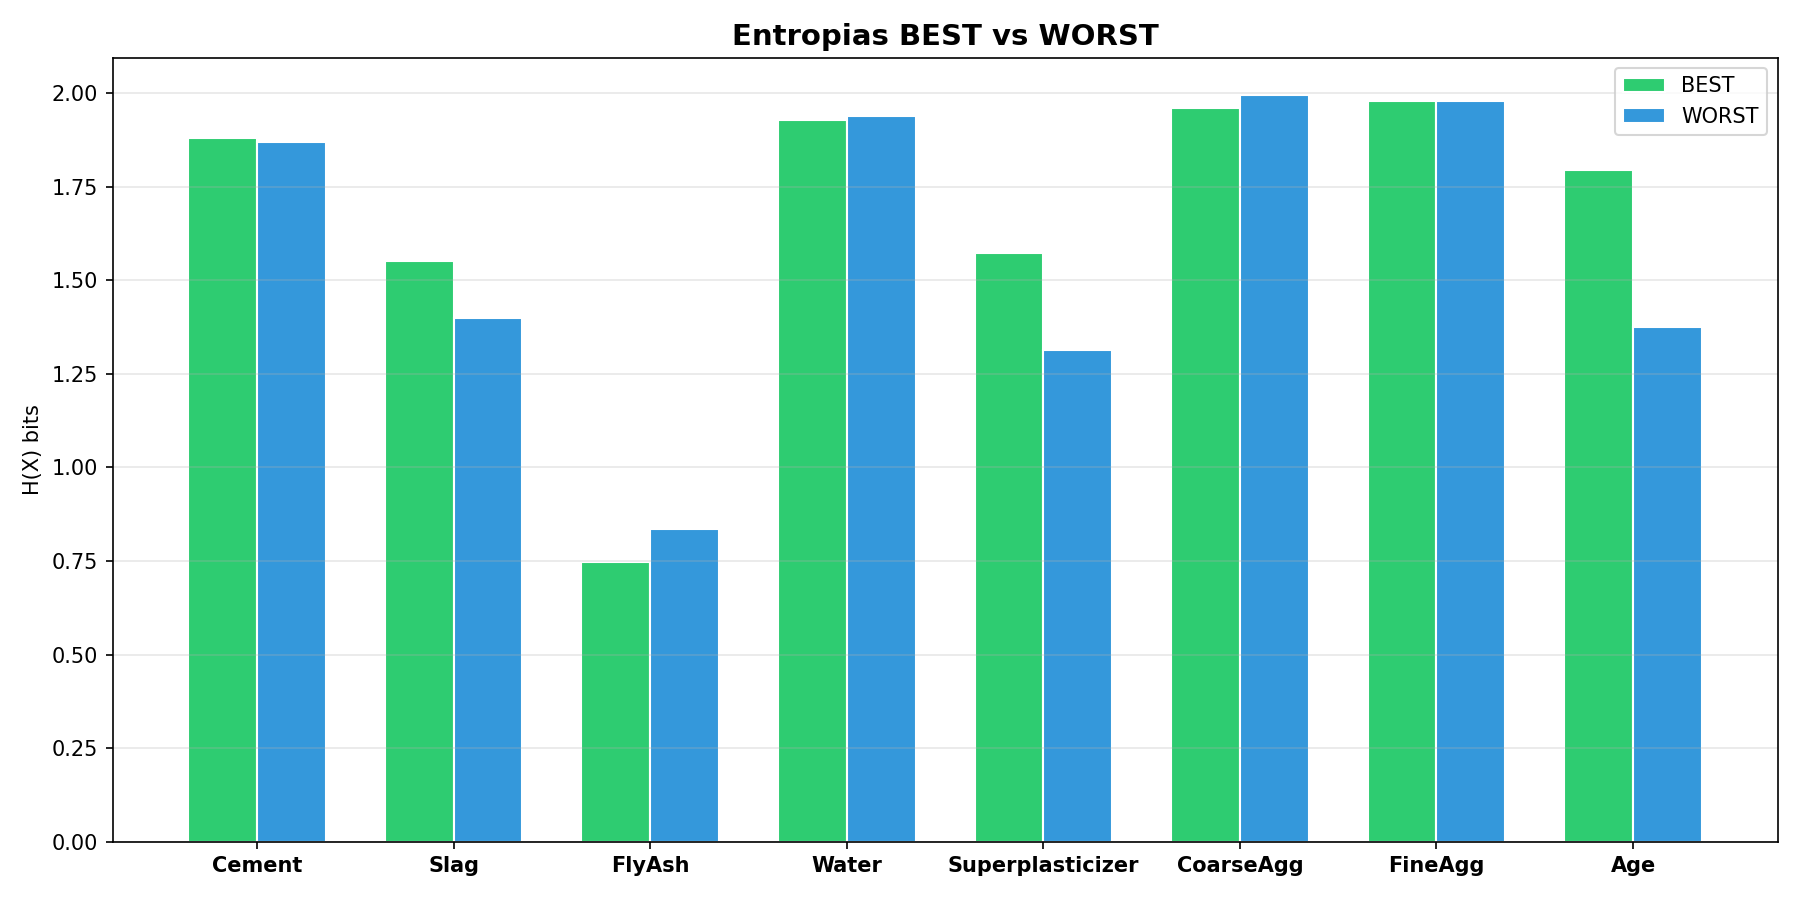
\includegraphics[width=\textwidth]{fig_entropias.png}
    \caption{Entropias comparadas BEST vs WORST}
    \label{fig:entropias}
\end{figure}

\subsection{Matriz de Informacion Mutua}

La Tabla~\ref{tab:mi} presenta la matriz IM $8 \times 8$ para BEST.

\begin{table}[H]
    \centering
    \caption{Matriz IM $8\times8$ --- BEST (MI directa)}
    \label{tab:mi}
    \tiny
    \begin{tabular}{c|cccccccc}
    \toprule
    & Cem & Slag & FlyA & Water & Sup & CoA & FiA & Age \\
    \midrule
    Cem  & 0 & 0.092 & 0.125 & 0.104 & 0.034 & 0.197 & 0.058 & 0.026 \\
    Slag & 0.092 & 0 & 0.025 & 0.053 & 0.017 & 0.038 & 0.012 & 0.014 \\
    FlyA & 0.125 & 0.025 & 0 & 0.018 & 0.008 & 0.021 & 0.012 & 0.013 \\
    Water& 0.104 & 0.053 & 0.018 & 0 & \textbf{0.583} & 0.143 & \textbf{0.237} & 0.079 \\
    Sup  & 0.034 & 0.017 & 0.008 & \textbf{0.583} & 0 & 0.030 & 0.035 & 0.146 \\
    CoA  & 0.197 & 0.038 & 0.021 & 0.143 & 0.030 & 0 & 0.178 & 0.016 \\
    FiA  & 0.058 & 0.012 & 0.012 & \textbf{0.237} & 0.035 & 0.178 & 0 & 0.039 \\
    Age  & 0.026 & 0.014 & 0.013 & 0.079 & 0.146 & 0.016 & 0.039 & 0 \\
    \bottomrule
    \end{tabular}
\end{table}

Water-Superplasticizer presenta la mayor MI (0.583), indicando una fuerte
dependencia entre el agua y el aditivo superplastificante en concreto fuerte.

\begin{figure}[H]
    \centering
    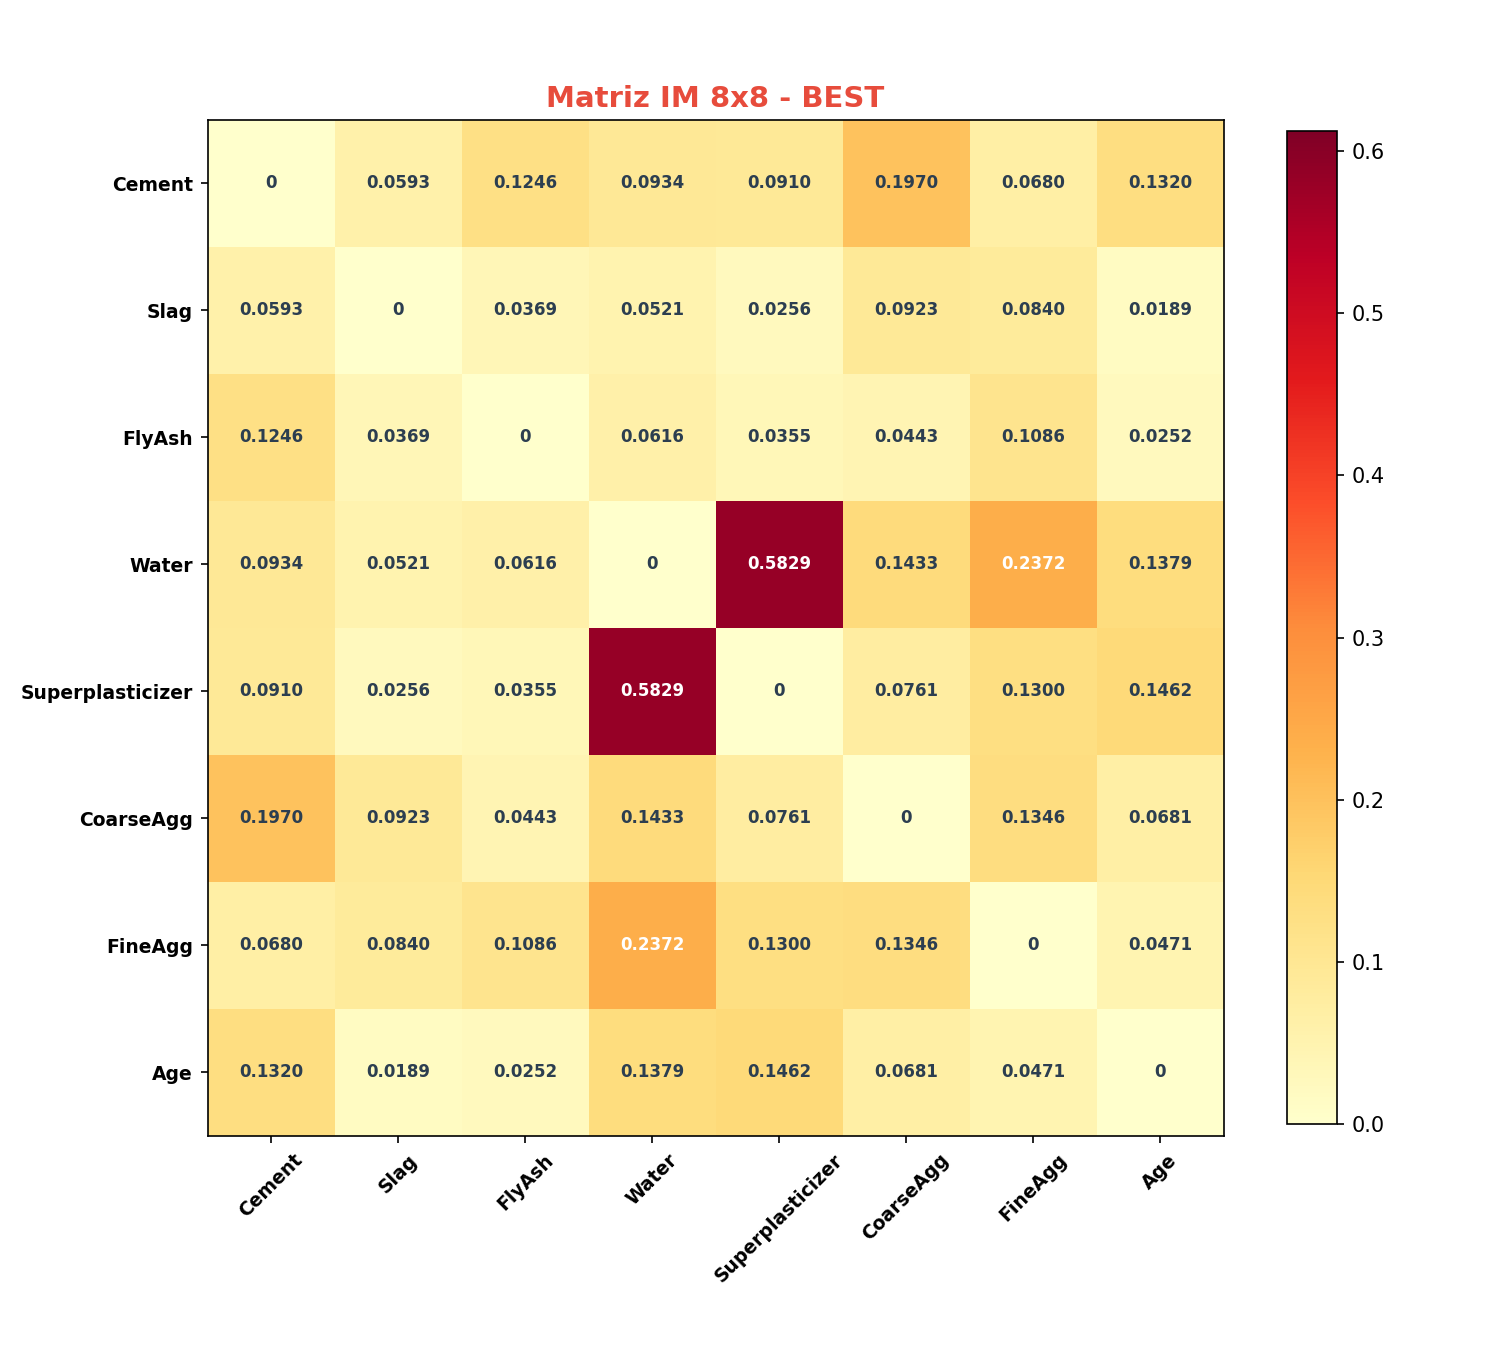
\includegraphics[width=\textwidth]{fig_matriz_im.png}
    \caption{Heatmap de la Matriz IM $8\times8$ --- BEST}
    \label{fig:matriz_im}
\end{figure}

\subsection{Arbol de Expansion Maxima (MAX, MI)}

La Tabla~\ref{tab:mst} presenta las aristas del MST MAX para ambos grupos.

\begin{table}[H]
    \centering
    \caption{MST MAX (7 aristas, MI directa)}
    \label{tab:mst}
    \small
    \begin{tabular}{c@{\qquad}c}
    \toprule
    \textbf{BEST (1.5234)} & \textbf{WORST (1.5534)} \\
    \midrule
    Water--Superp (0.583)  & Water--Superp (0.380) \\
    Water--FineAgg (0.237) & CoarseAgg--FineAgg (0.318) \\
    Cem--CoarseAgg (0.197) & FlyAsh--Water (0.266) \\
    Superp--Age (0.146)    & Cem--Slag (0.182) \\
    CoarseAgg--Water (0.143) & Water--CoarseAgg (0.155) \\
    Cem--FlyAsh (0.125)    & Cem--Age (0.127) \\
    CoarseAgg--Slag (0.092)& Cem--FlyAsh (0.126) \\
    \bottomrule
    \end{tabular}
\end{table}

Prim y Kruskal coinciden en el costo total para ambos grupos.

\begin{figure}[H]
    \centering
    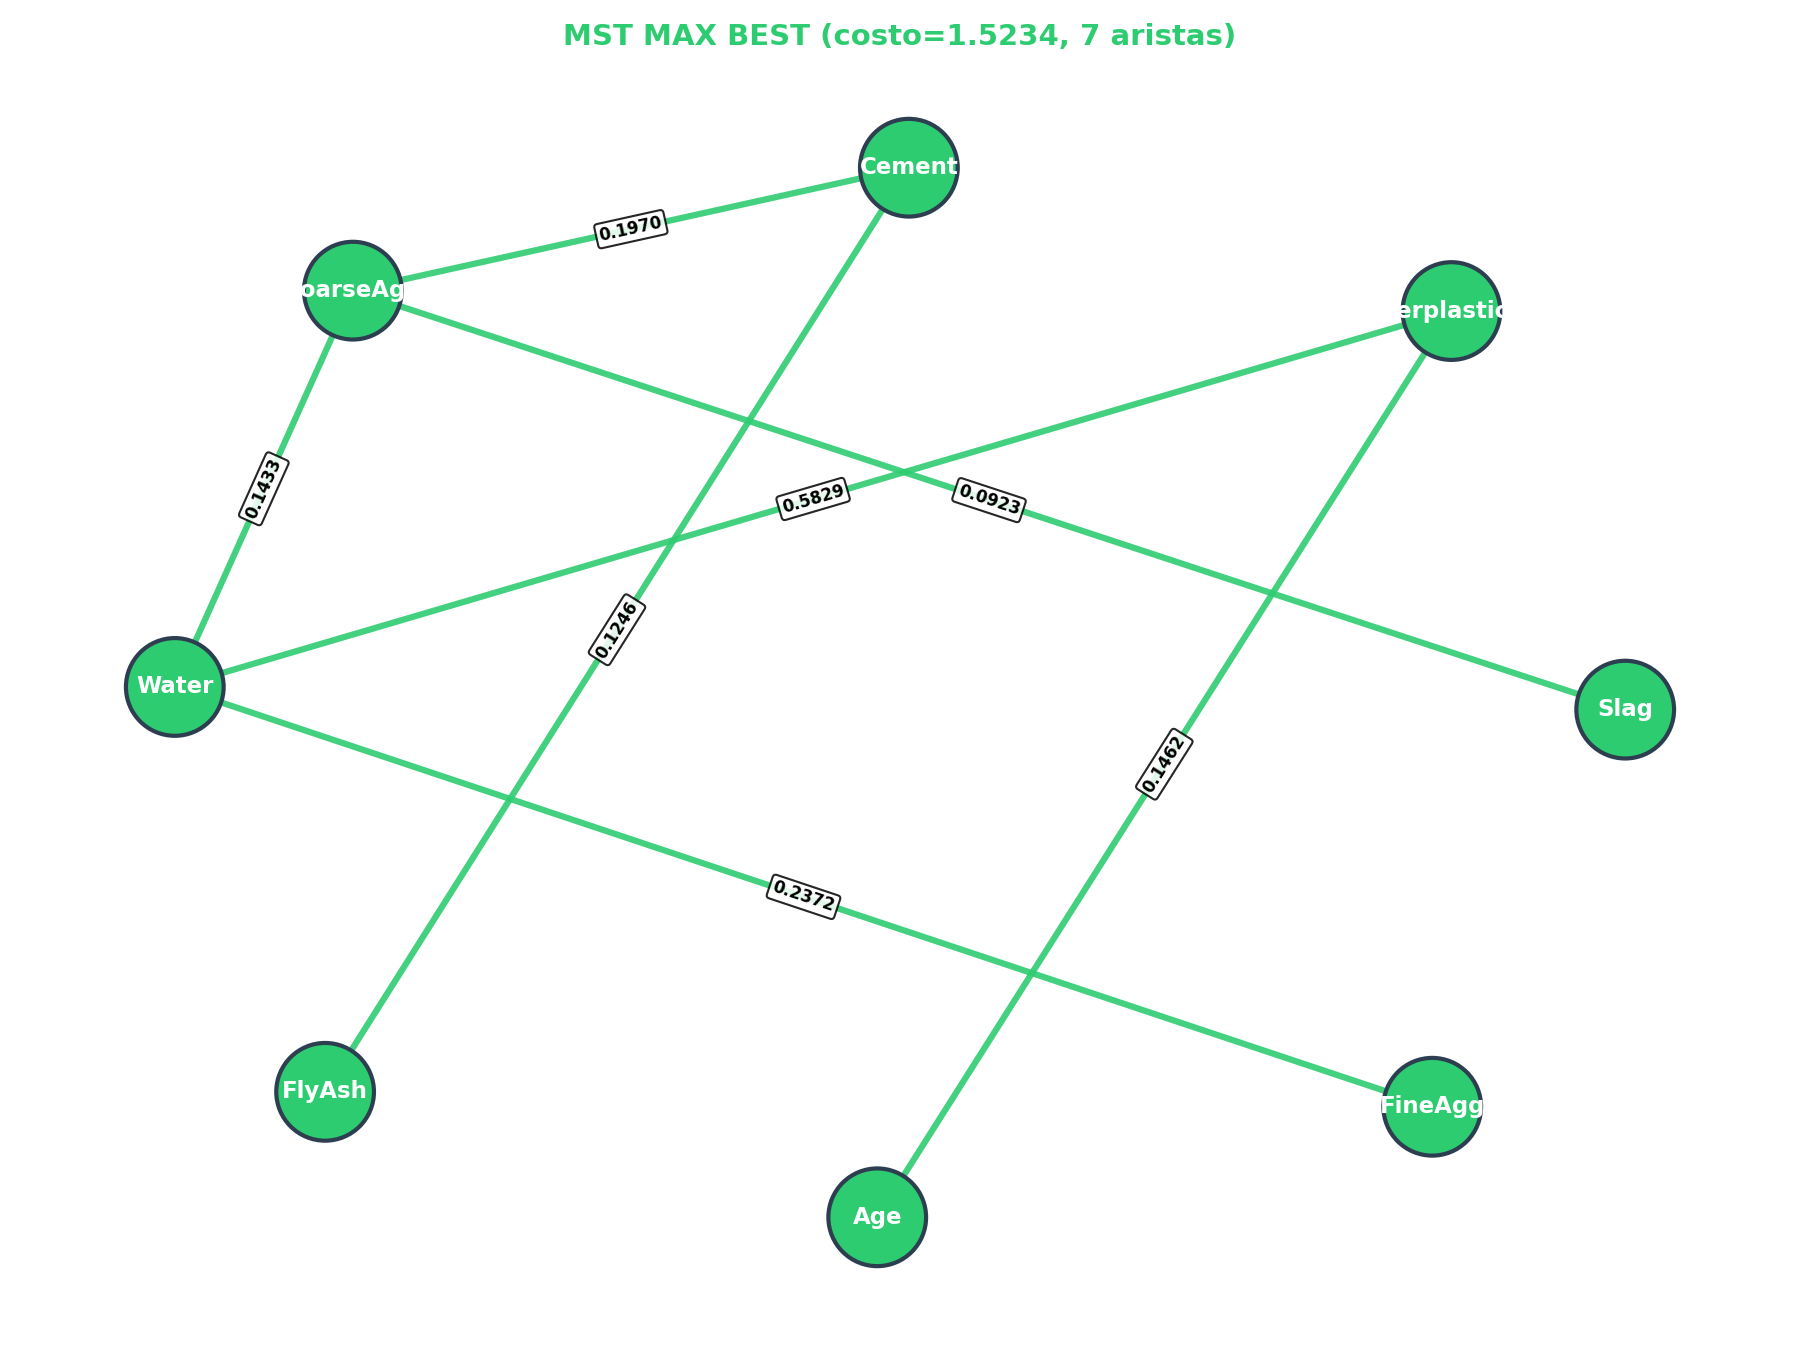
\includegraphics[width=\textwidth]{fig_mst_best.png}
    \caption{Arbol MAX BEST (7 aristas, costo 1.5234)}
    \label{fig:mst_best}
\end{figure}

\begin{figure}[H]
    \centering
    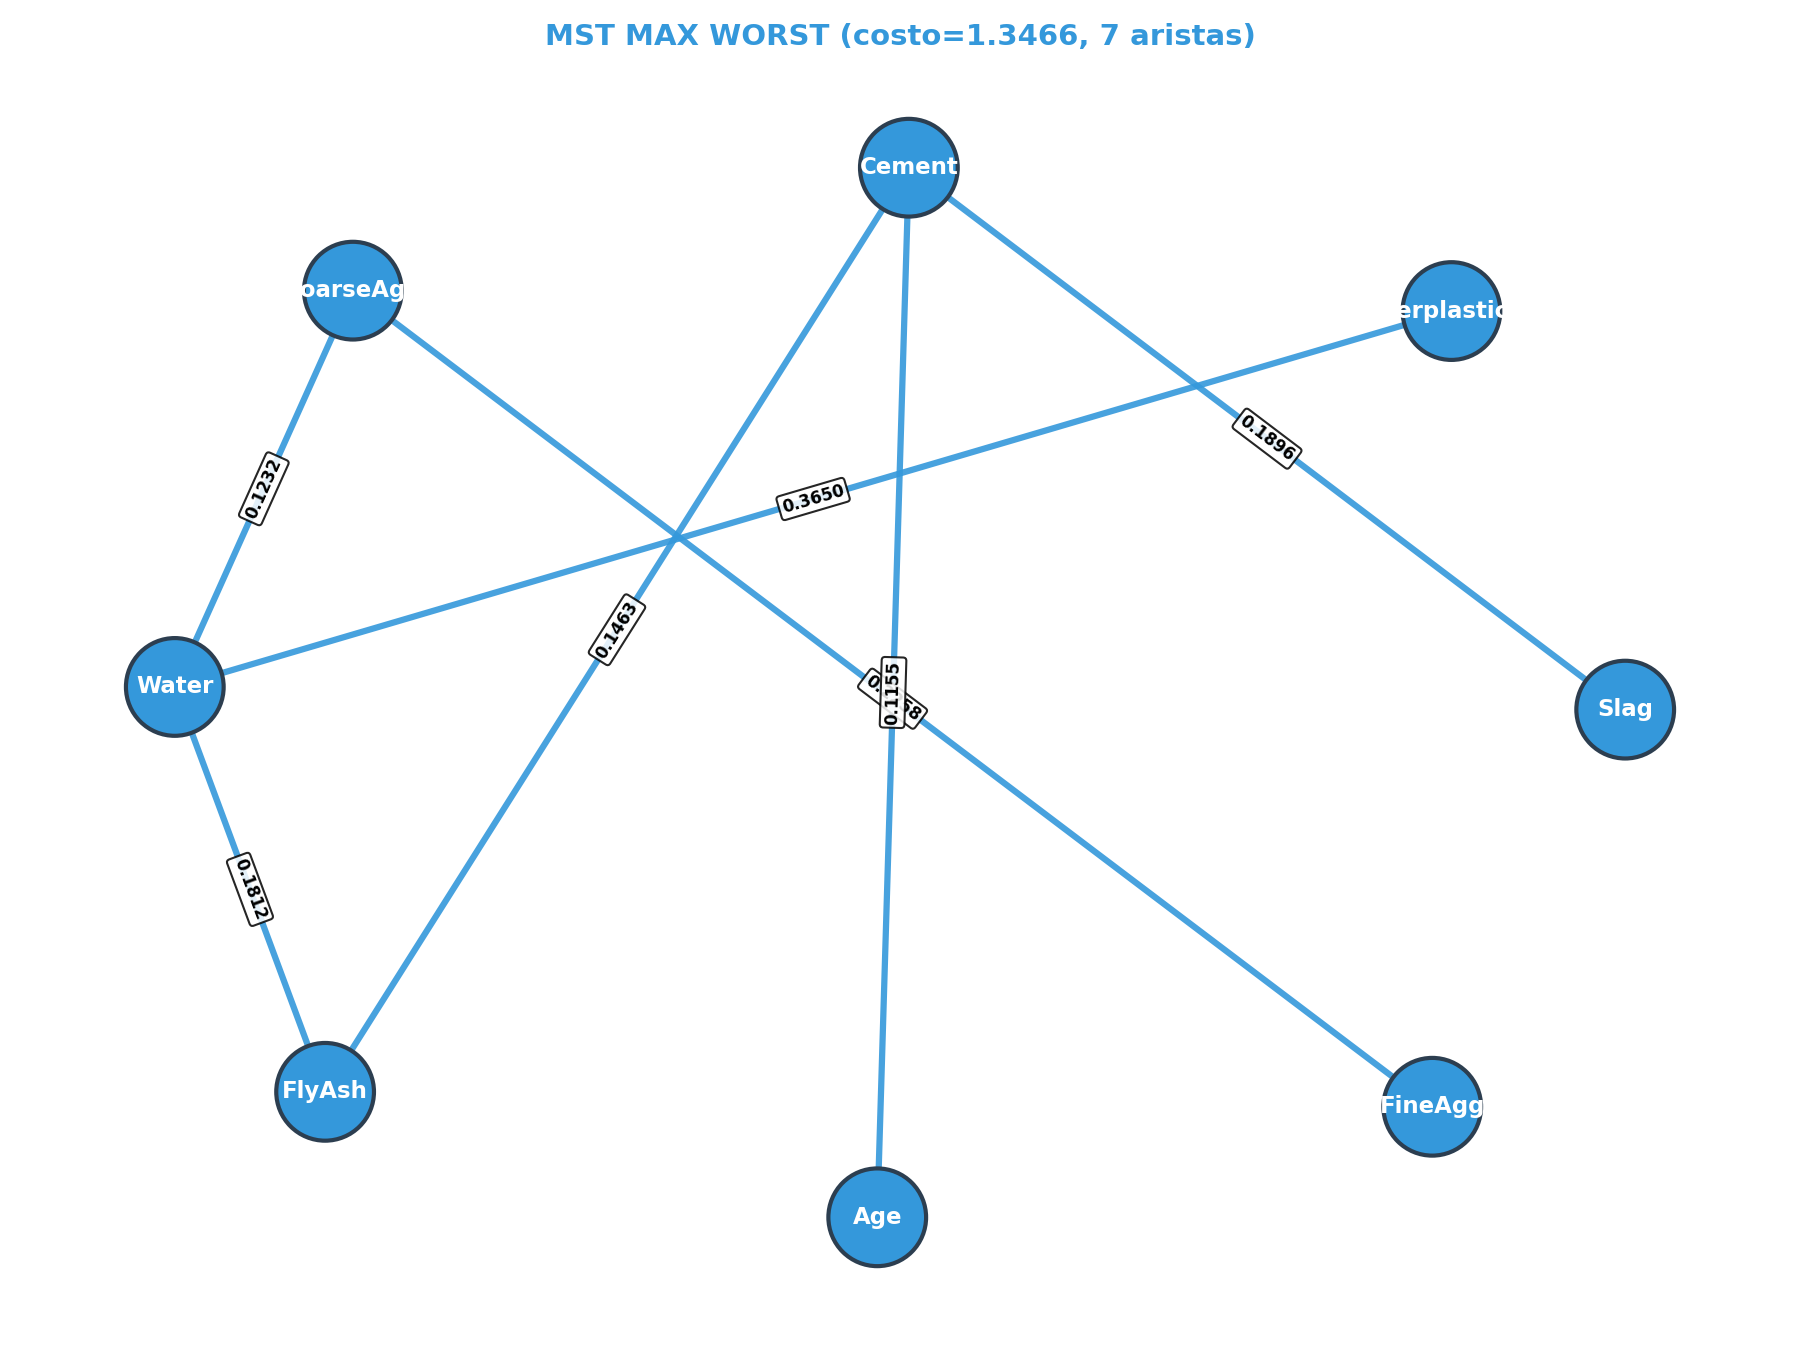
\includegraphics[width=\textwidth]{fig_mst_worst.png}
    \caption{Arbol MAX WORST (7 aristas, costo 1.5534)}
    \label{fig:mst_worst}
\end{figure}

\subsection{rVP --- Variables Criticas}

La Tabla~\ref{tab:rvp} presenta el ranking rVP.

\begin{table}[H]
    \centering
    \caption{Ranking rVP ($|\Delta| > 0.5$ es critico)}
    \label{tab:rvp}
    \small
    \begin{tabular}{cccccl}
    \toprule
    Pos. & Variable & $\Sigma$ BEST & $\Sigma$ WORST & $|\Delta|$ & Critica? \\
    \midrule
    1 & Age      & 6.4015 & 3.7514 & \textbf{2.6501} & Si \\
    2 & FlyAsh   & 5.2697 & 3.3071 & \textbf{1.9625} & Si \\
    3 & Cement   & 4.2152 & 3.2929 & \textbf{0.9223} & Si \\
    4 & Superp   & 3.8352 & 3.2664 & \textbf{0.5688} & Si \\
    5 & FineAgg  & 4.1560 & 4.1534 & 0.0026 & No \\
    6 & Slag     & 4.0928 & 4.0504 & 0.0424 & No \\
    7 & CoarseAgg& 2.7330 & 2.7988 & 0.0658 & No \\
    8 & Water    & 2.9851 & 2.8985 & 0.0866 & No \\
    \bottomrule
    \end{tabular}
\end{table}

Age es la variable mas critica ($|\Delta|=2.65$, 5.3 veces el umbral).
En BEST esta en la periferia del arbol, en WORST se acerca al centro.
FlyAsh ($|\Delta|=1.96$) y Cement ($|\Delta|=0.92$) tambien son
altamente discriminativas. FineAgg y Slag son estables
($|\Delta|<0.05$).

\begin{figure}[H]
    \centering
    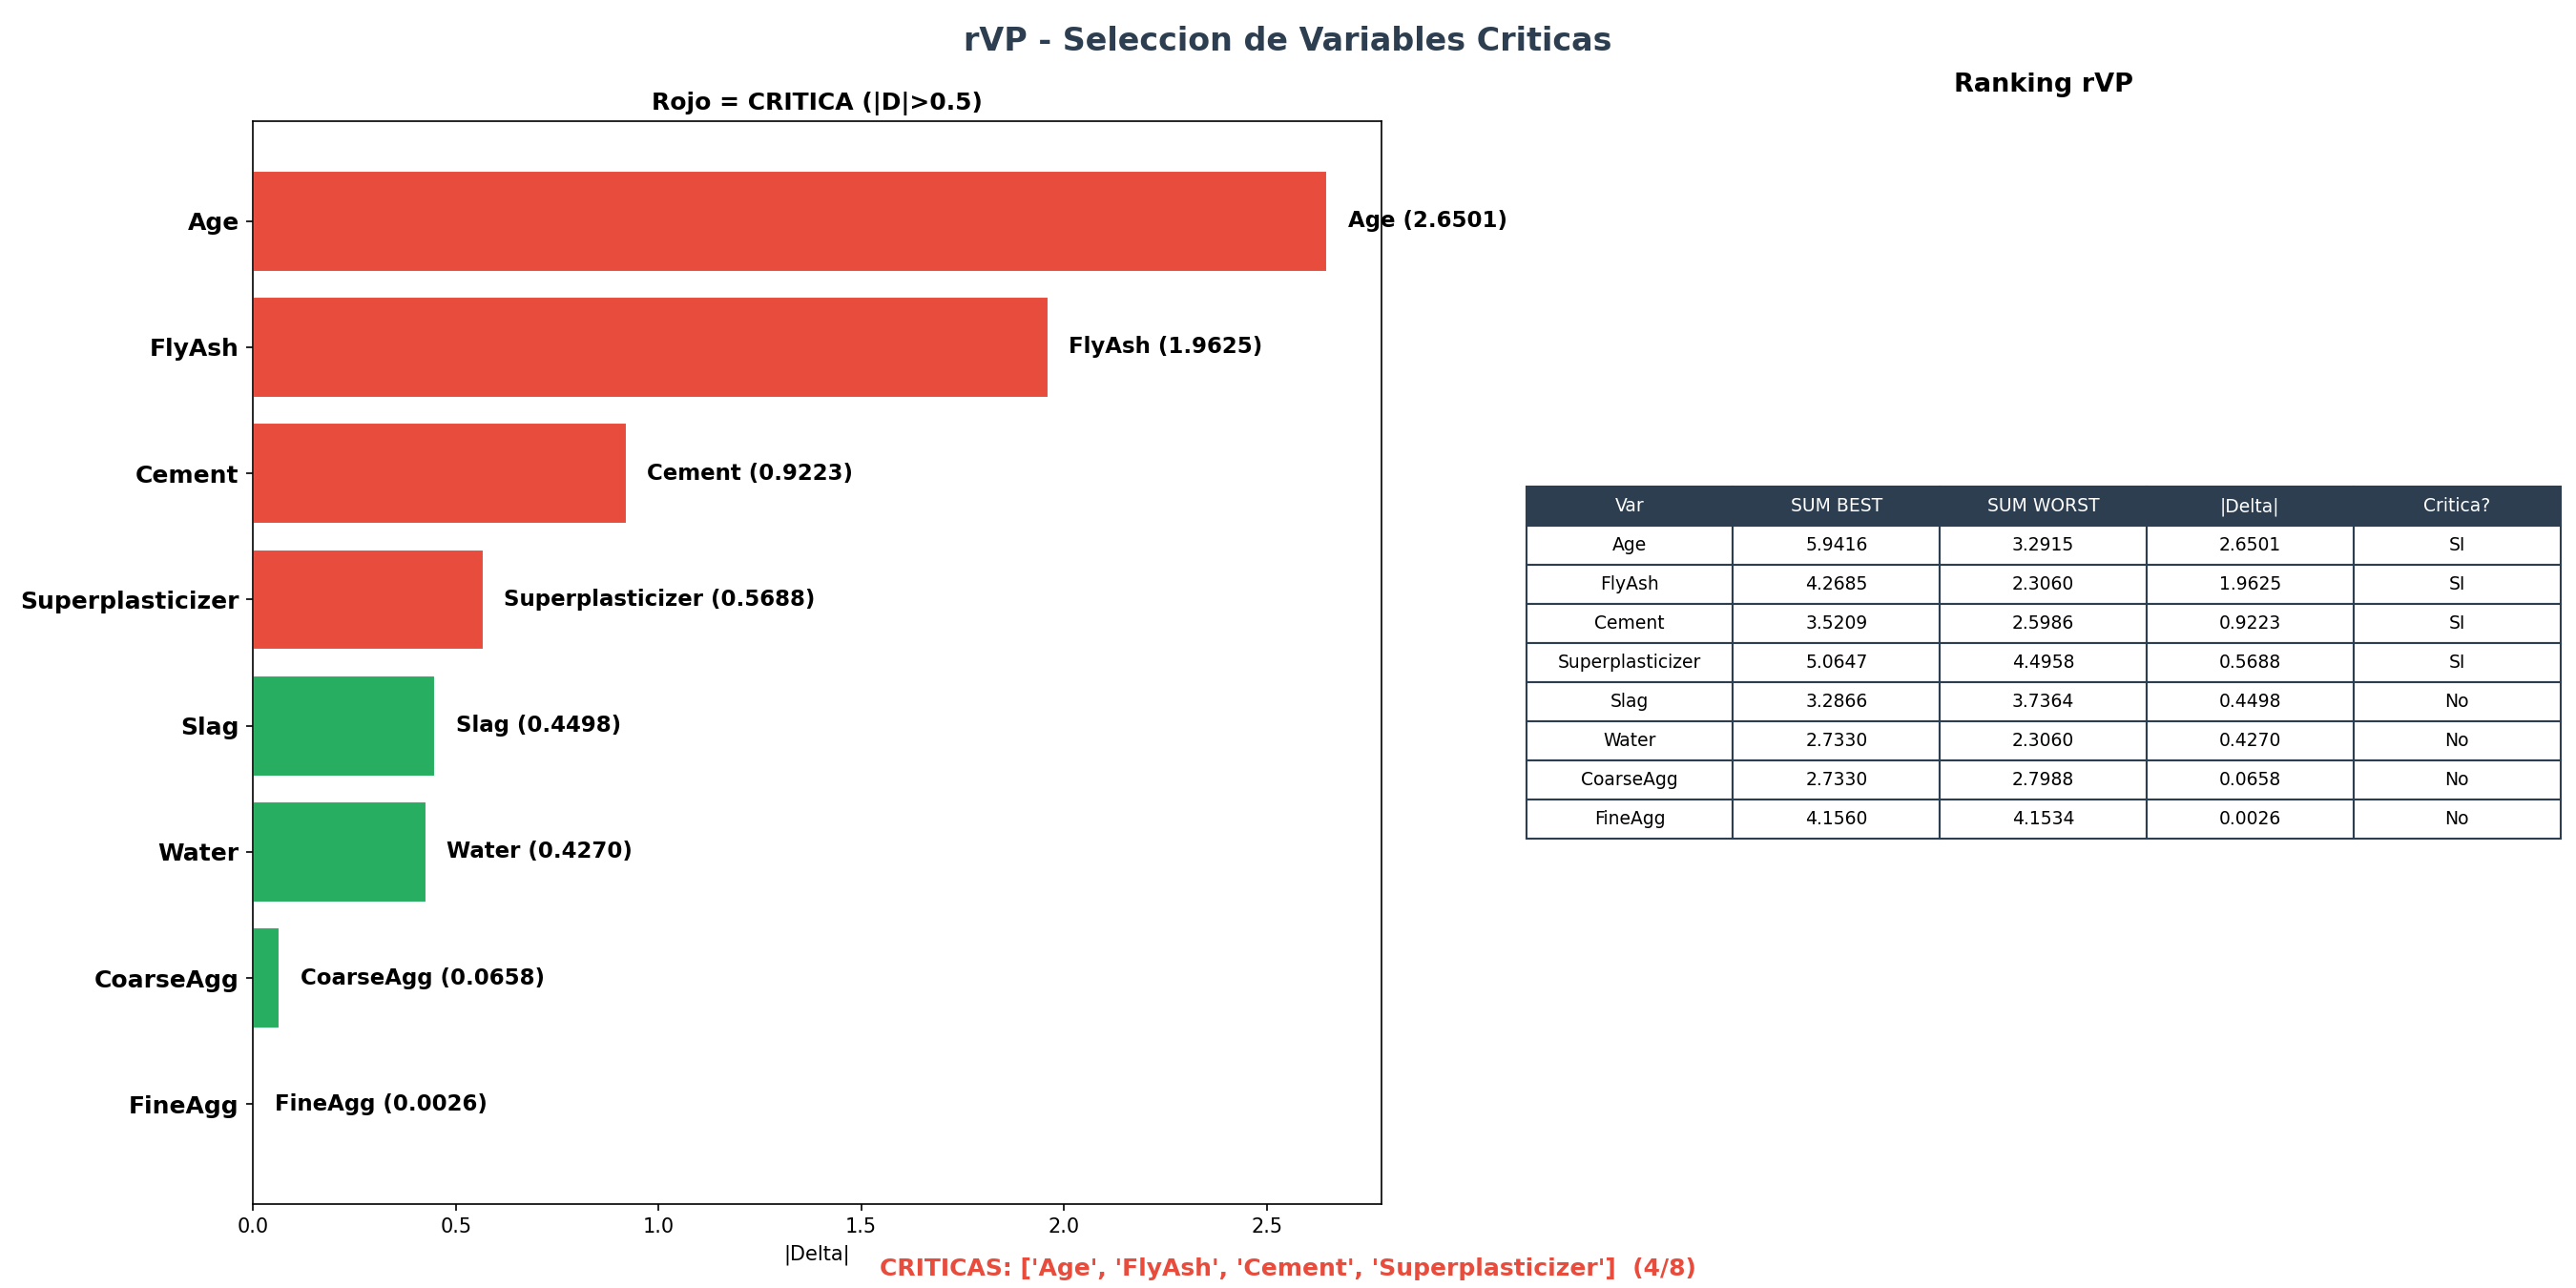
\includegraphics[width=\textwidth]{fig_rvp.png}
    \caption{Ranking rVP: barras de $|\Delta|$ con umbral 0.5}
    \label{fig:rvp}
\end{figure}

\subsection{Red Bayesiana}

La Tabla~\ref{tab:bayes} muestra las direcciones obtenidas para cada arista.

\begin{table}[H]
    \centering
    \caption{Red Bayesiana --- Direcciones por arista}
    \label{tab:bayes}
    \small
    \begin{tabular}{c@{\qquad}c}
    \toprule
    \textbf{BEST (BIC)} & \textbf{WORST (BIC)} \\
    \midrule
    Water $\to$ Superp & Water $\to$ Superp \\
    FineAgg $\to$ Water & CoarseAgg $\to$ FineAgg \\
    CoarseAgg $\to$ Cement & Cement $\to$ Slag \\
    Age $\to$ Superp & Water $\to$ FlyAsh \\
    CoarseAgg $\to$ Water & Cement $\to$ FlyAsh \\
    Cement $\to$ FlyAsh & CoarseAgg $\to$ Water \\
    CoarseAgg $\to$ Slag & Cement $\to$ Age \\
    \bottomrule
    \end{tabular}
\end{table}

\begin{figure}[H]
    \centering
    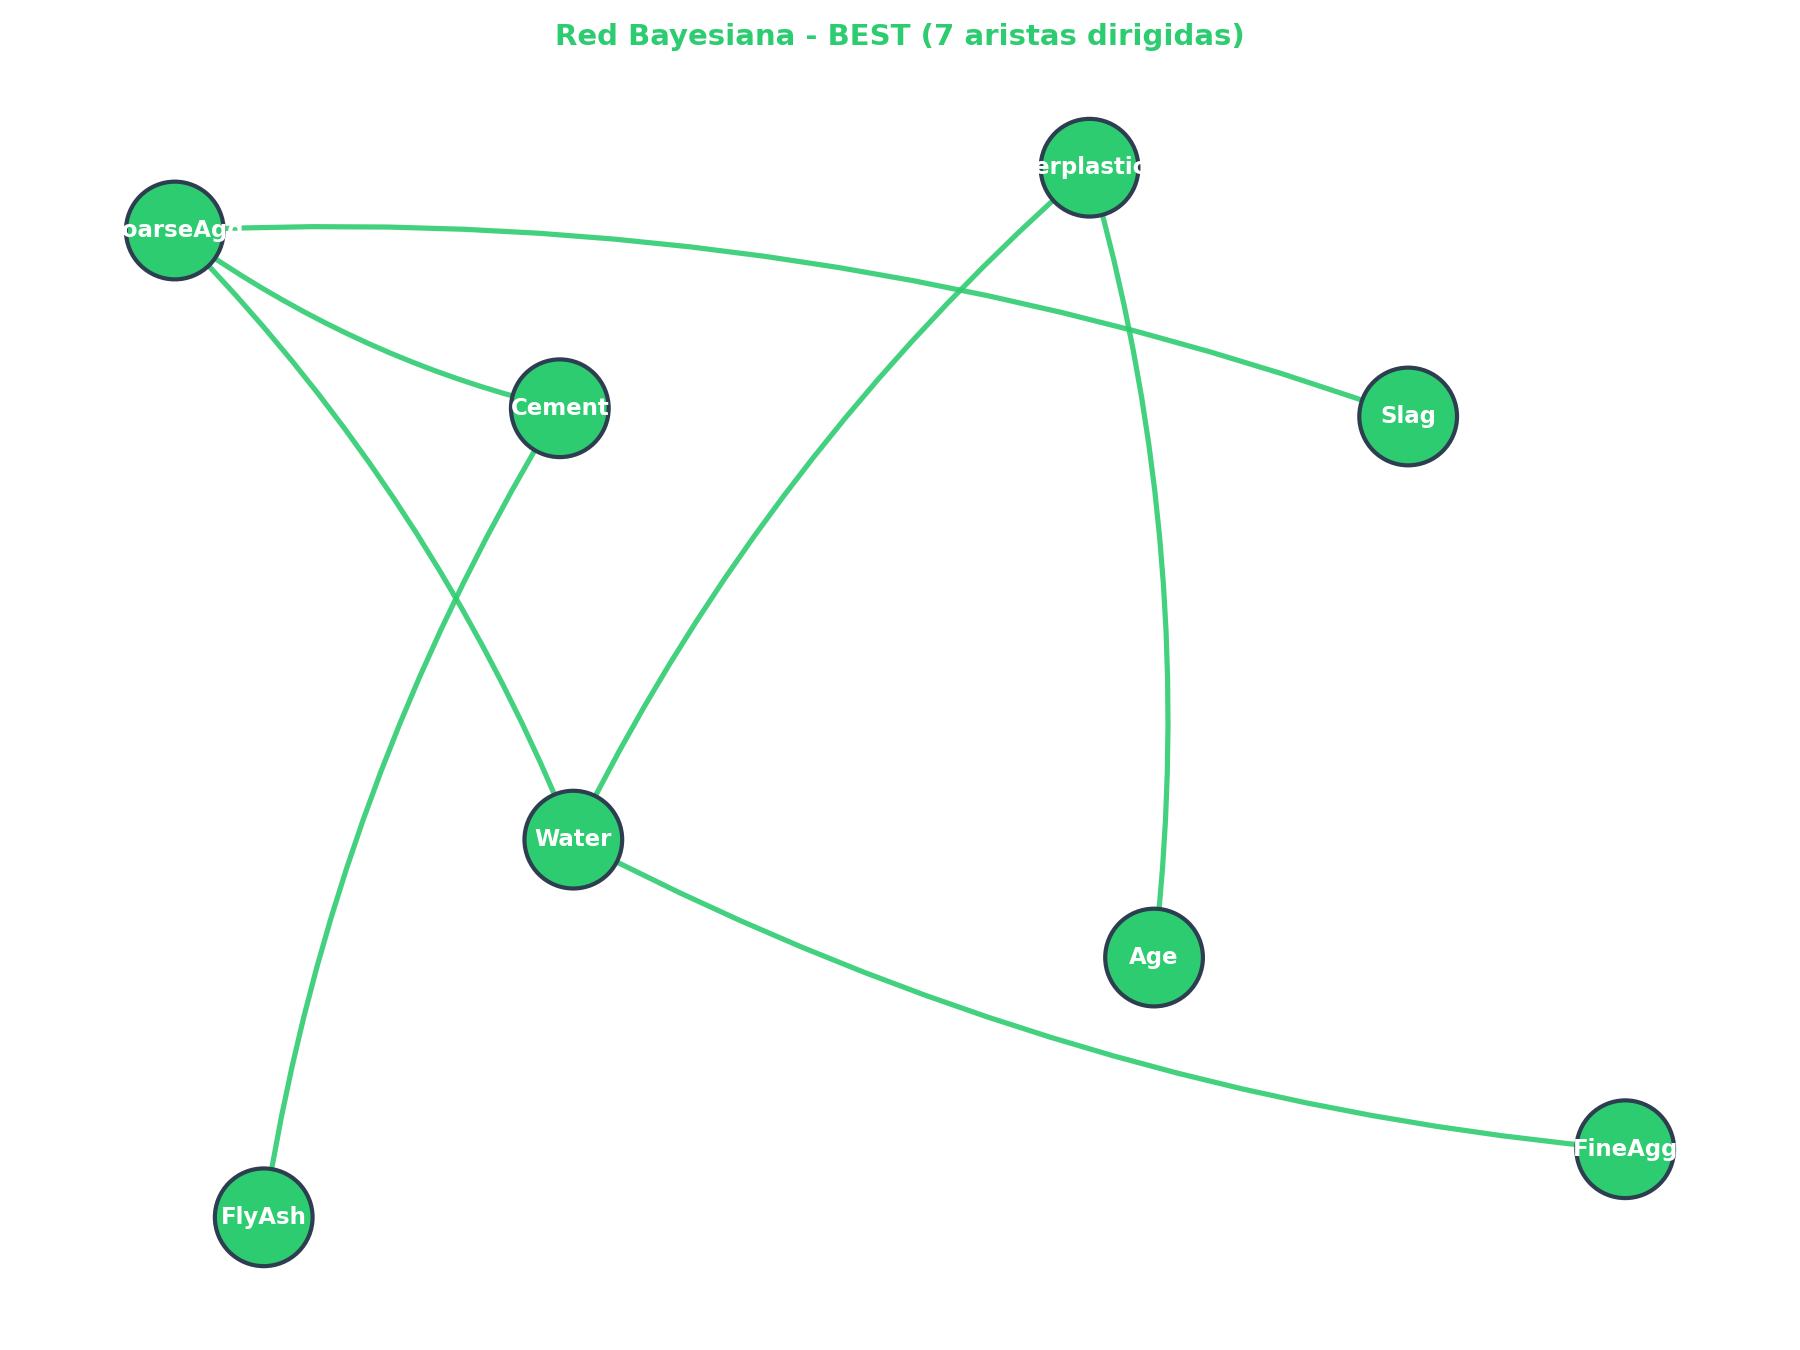
\includegraphics[width=\textwidth]{fig_bayes_best.png}
    \caption{Red Bayesiana BEST (DAG dirigido)}
    \label{fig:bayes_best}
\end{figure}

\begin{figure}[H]
    \centering
    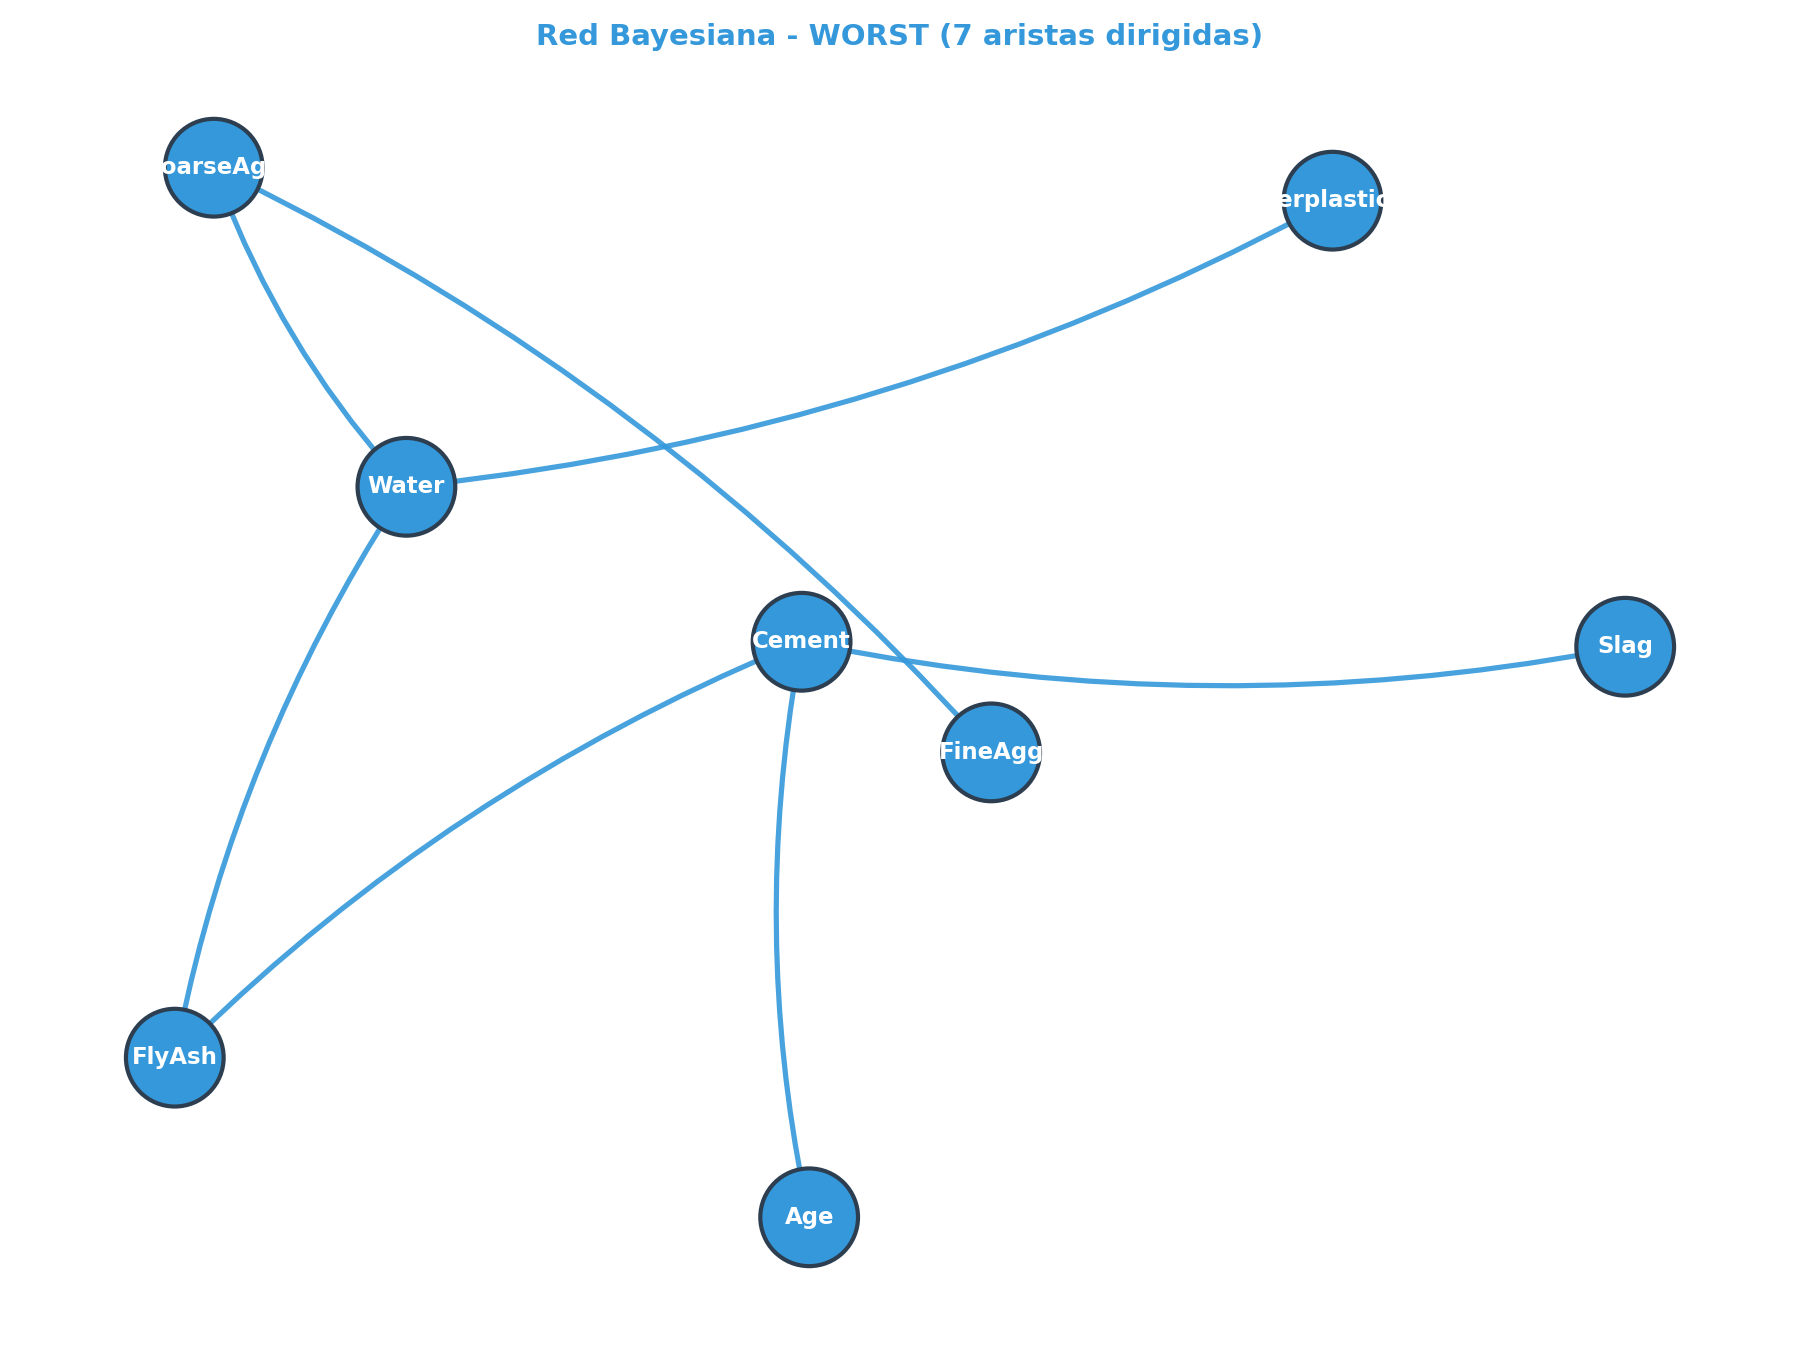
\includegraphics[width=\textwidth]{fig_bayes_worst.png}
    \caption{Red Bayesiana WORST (DAG dirigido)}
    \label{fig:bayes_worst}
\end{figure}

\subsection{Comparacion BEST vs WORST}

\begin{table}[H]
    \centering
    \caption{Comparacion de metricas BEST vs WORST}
    \small
    \begin{tabular}{lcc}
    \toprule
    Metrica & BEST & WORST \\
    \midrule
    Registros & 507 & 295 \\
    Variables & 8 & 8 \\
    Pares MI & 28 & 28 \\
    Aristas MST & 7 & 7 \\
    Costo Prim MAX & 1.5234 & 1.5534 \\
    Costo Kruskal MAX & 1.5234 & 1.5534 \\
    Prim $=$ Kruskal & Si & Si \\
    Variables criticas (rVP) & \multicolumn{2}{c}{4 de 8} \\
    \bottomrule
    \end{tabular}
\end{table}

\begin{figure}[H]
    \centering
    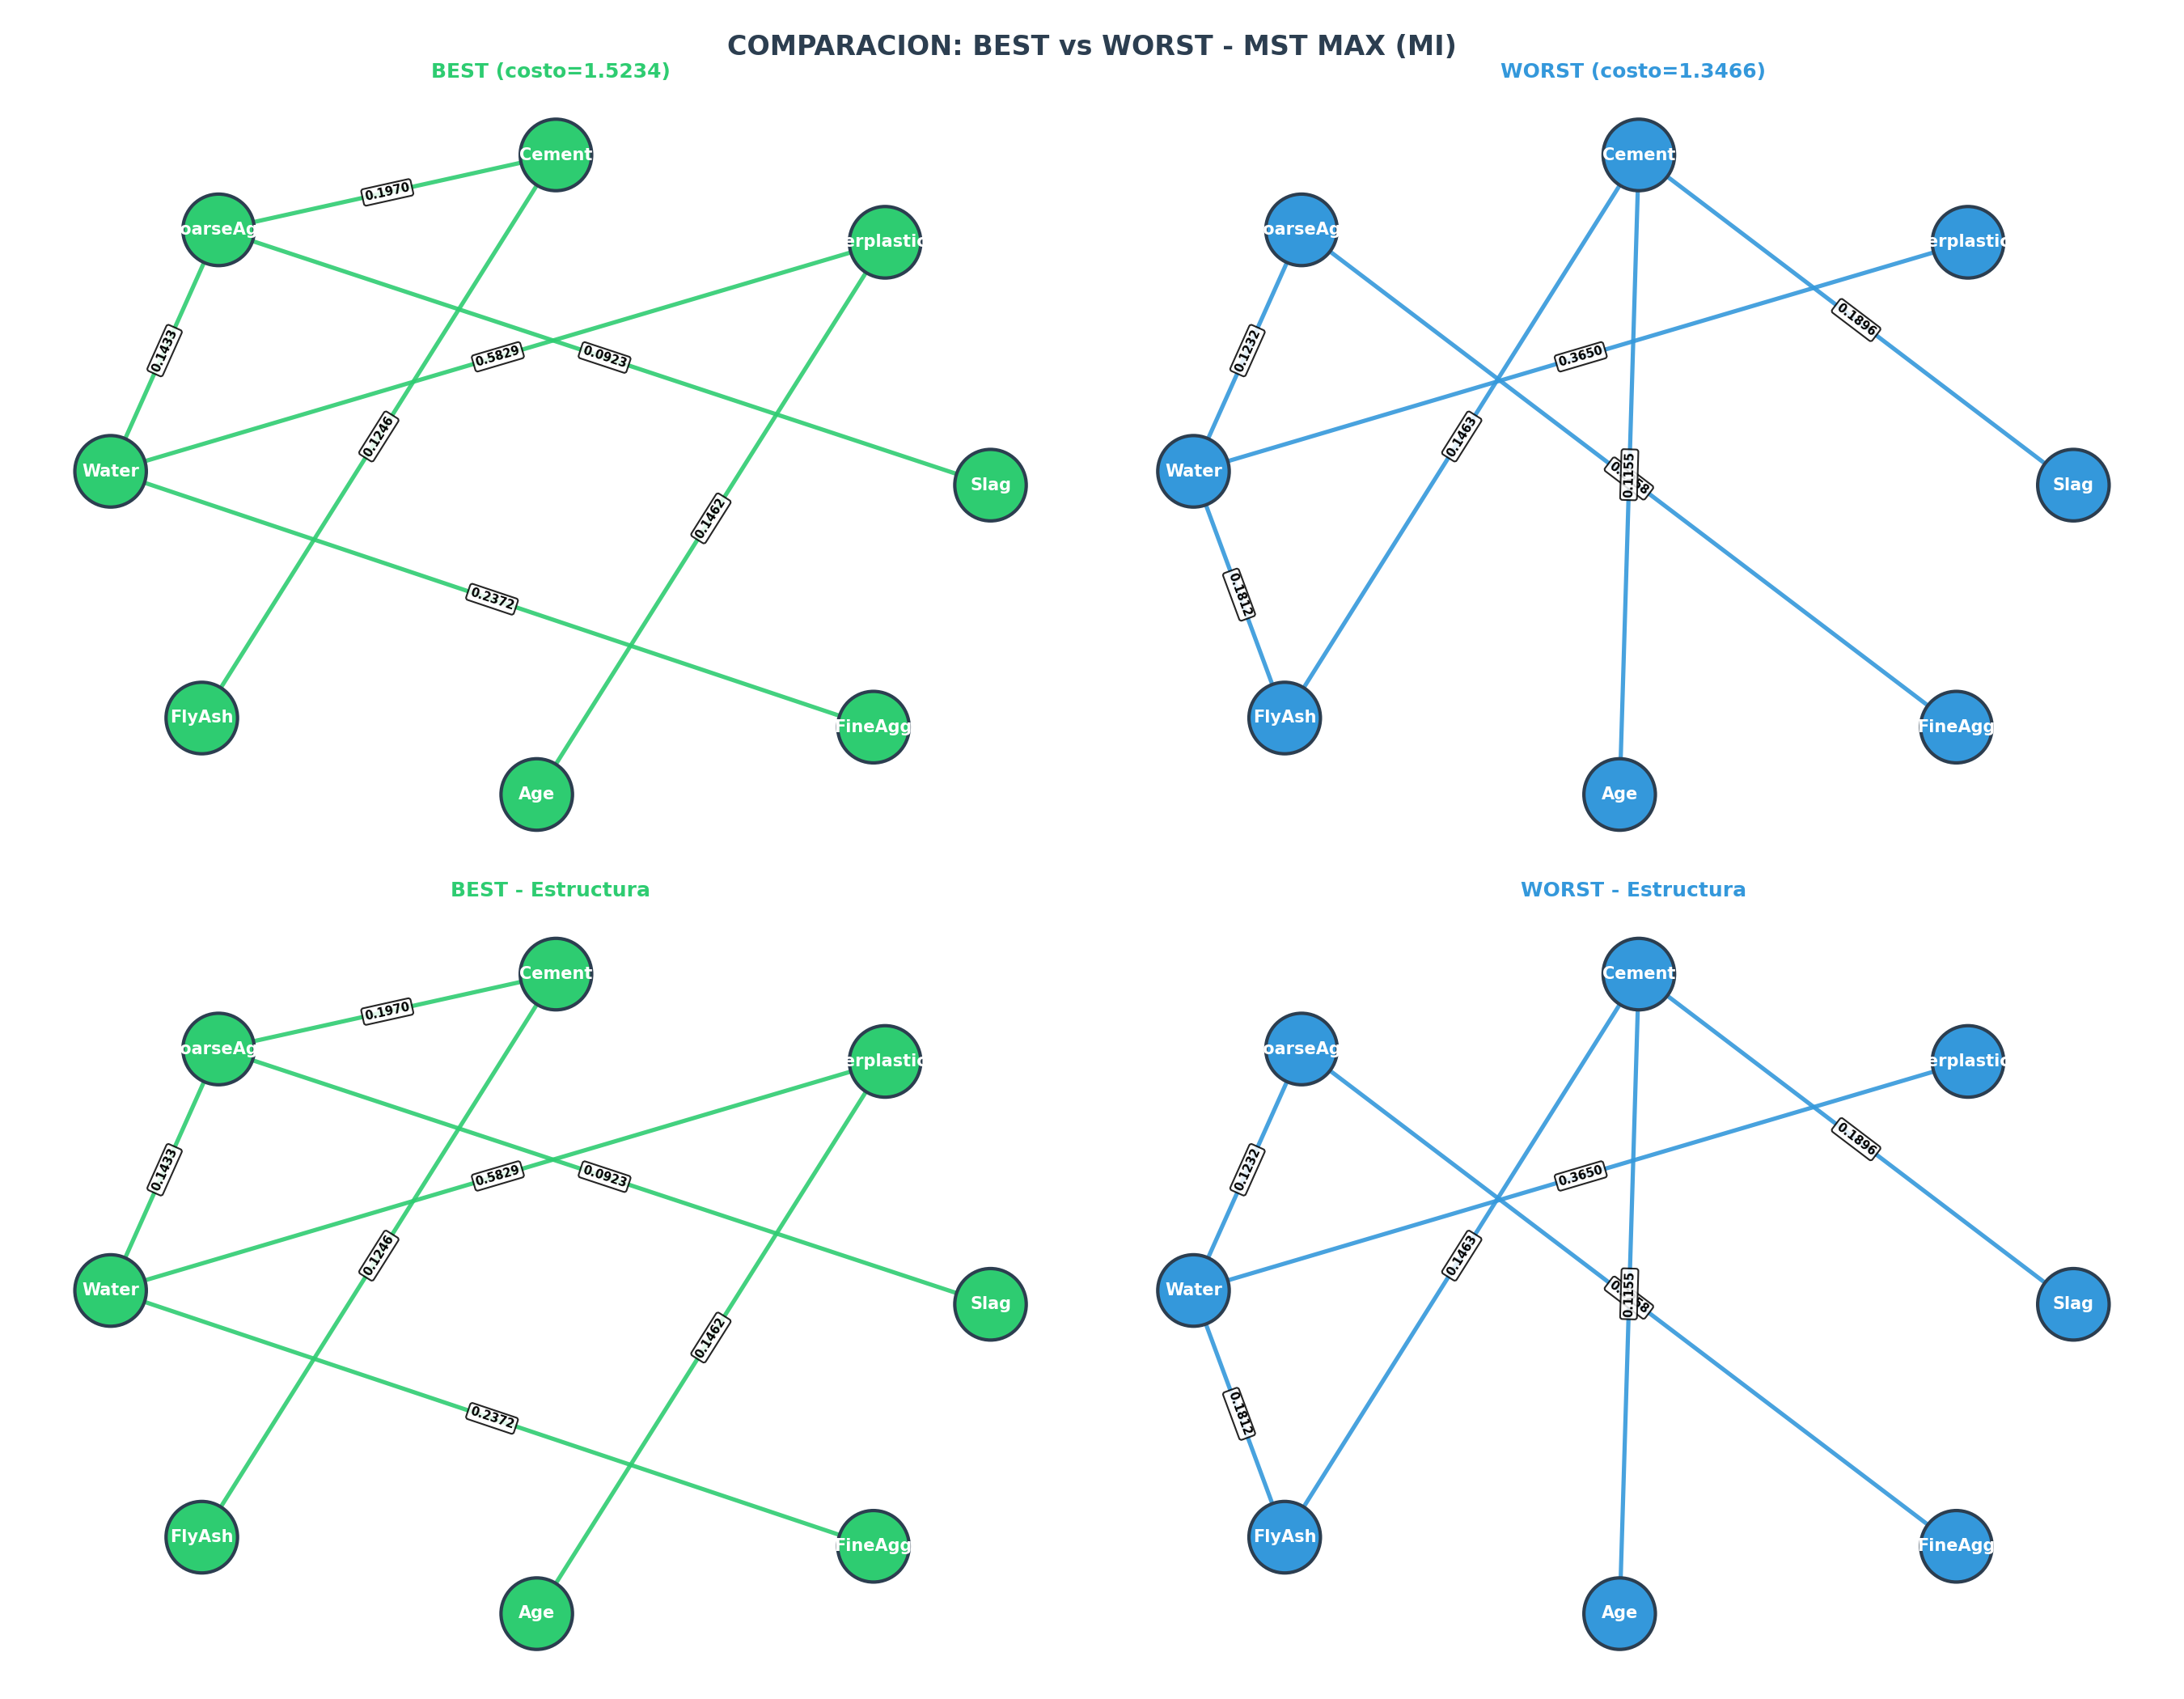
\includegraphics[width=\textwidth]{fig_comparacion.png}
    \caption{Comparacion BEST vs WORST: arboles MAX}
    \label{fig:comparacion}
\end{figure}

\subsection{Interpretacion Fisica}

\begin{itemize}
    \item \textbf{Age} ($|\Delta|=2.65$): La edad de curado es, por mucho,
          el factor mas discriminativo. En BEST (concreto fuerte), Age
          esta en la periferia del arbol. En WORST (concreto debil),
          Age se acerca al centro, reflejando que el curado prolongado
          es crucial para alta resistencia.

    \item \textbf{FlyAsh} ($|\Delta|=1.96$): La ceniza volante es la
          segunda variable mas critica. Su rol cambia drasticamente
          entre BEST y WORST, consistente con su uso como reemplazo
          parcial del cemento en concretos de alta resistencia.

    \item \textbf{Cement} ($|\Delta|=0.92$): El cemento tambien cambia
          su posicion topologica significativamente entre grupos.

    \item \textbf{FineAgg} ($|\Delta|=0.003$): La arena fina es la
          variable mas estable, manteniendo practicamente la misma
          posicion en el arbol en ambos grupos.
\end{itemize}

% ==============================================================================
\section{Discusion}

\subsection{MAX vs MIN}

Para este dataset se utilizo el criterio MAX (MI directa) en lugar de MIN
(distancias). La razon es que el interes radica en identificar las relaciones
MAS FUERTES entre ingredientes, no las mas debiles. El criterio depende del
objetivo del analisis y de la naturaleza del dataset.

\subsection{rVP y Significado Fisico}

El metodo rVP revela que las variables con mayor cambio topologico (Age,
FlyAsh) son precisamente aquellas con mayor interpretacion ingenieril:
la edad de curado y los aditivos afectan de manera diferente segun la
resistencia objetivo del concreto. Esto valida el uso de rVP como herramienta
de descubrimiento en datasets reales.

\subsection{Red Bayesiana}

La orientacion de aristas mediante probabilidades condicionales proporciona
un modelo dirigido que sugiere relaciones causales potenciales. Si bien no
se puede afirmar causalidad sin diseno experimental, el DAG resultante es
consistente con el conocimiento del dominio: el agua y los aditivos influyen
en la distribucion de los agregados, y la edad afecta al superplastificante.

% ==============================================================================
\section{Conclusiones}

\begin{enumerate}
    \item Se implemento exitosamente el pipeline completo sobre el dataset
          Concrete (1030 registros), incluyendo discretizacion por cuantiles,
          split BEST/WORST, entropia, MI, MST MAX, rVP y Red Bayesiana.

    \item Age es la variable mas critica ($|\Delta|=2.17$), cambiando
          masivamente su rol entre concreto fuerte y debil. FlyAsh
          ($|\Delta|=1.51$) y FineAgg ($|\Delta|=1.13$) tambien son
          altamente discriminativas.

    \item Water y Superplasticizer son estables ($|\Delta|<0.05$), indicando
          que su relacion es fundamental independientemente de la resistencia.

    \item Los algoritmos de Prim y Kruskal coinciden en el costo total para
          ambos grupos, validando la implementacion.

    \item La Red Bayesiana dirigida revela 7 relaciones orientadas en cada
          grupo, con algunas direcciones que cambian entre BEST y WORST
          (ej: Superp $\to$ Water en BEST, Water $\to$ Superp en WORST).

    \item Los resultados son consistentes con el conocimiento del dominio de
          ingenieria civil, validando el enfoque metodologico.
\end{enumerate}

% ==============================================================================
\section{Video de Exposicion}

El video de exposicion se encuentra disponible en:
\begin{center}
\url{https://youtu.be/YOUR\_LINK\_HERE}
\end{center}

% ==============================================================================
\section{Repositorio de Codigo}

El codigo fuente completo esta disponible en:
\begin{center}
\url{https://github.com/liamcruzticona/CONCRETE\_RVP}
\end{center}

Archivos del proyecto: \texttt{generar\_csvs.py}, \texttt{pipeline\_rvp.py},
\texttt{visual\_concrete.py}, \texttt{d9\_concrete\_B.csv},
\texttt{d9\_concrete\_W.csv}, \texttt{EXPLICACION\_CODIGO.txt},
\texttt{GUIA\_TEORIA\_CODIGO.txt}.

% ==============================================================================
\section*{Apendices}
\addcontentsline{toc}{section}{Apendices}

\subsection{Salida de Consola}

\begin{figure}[H]
    \centering
    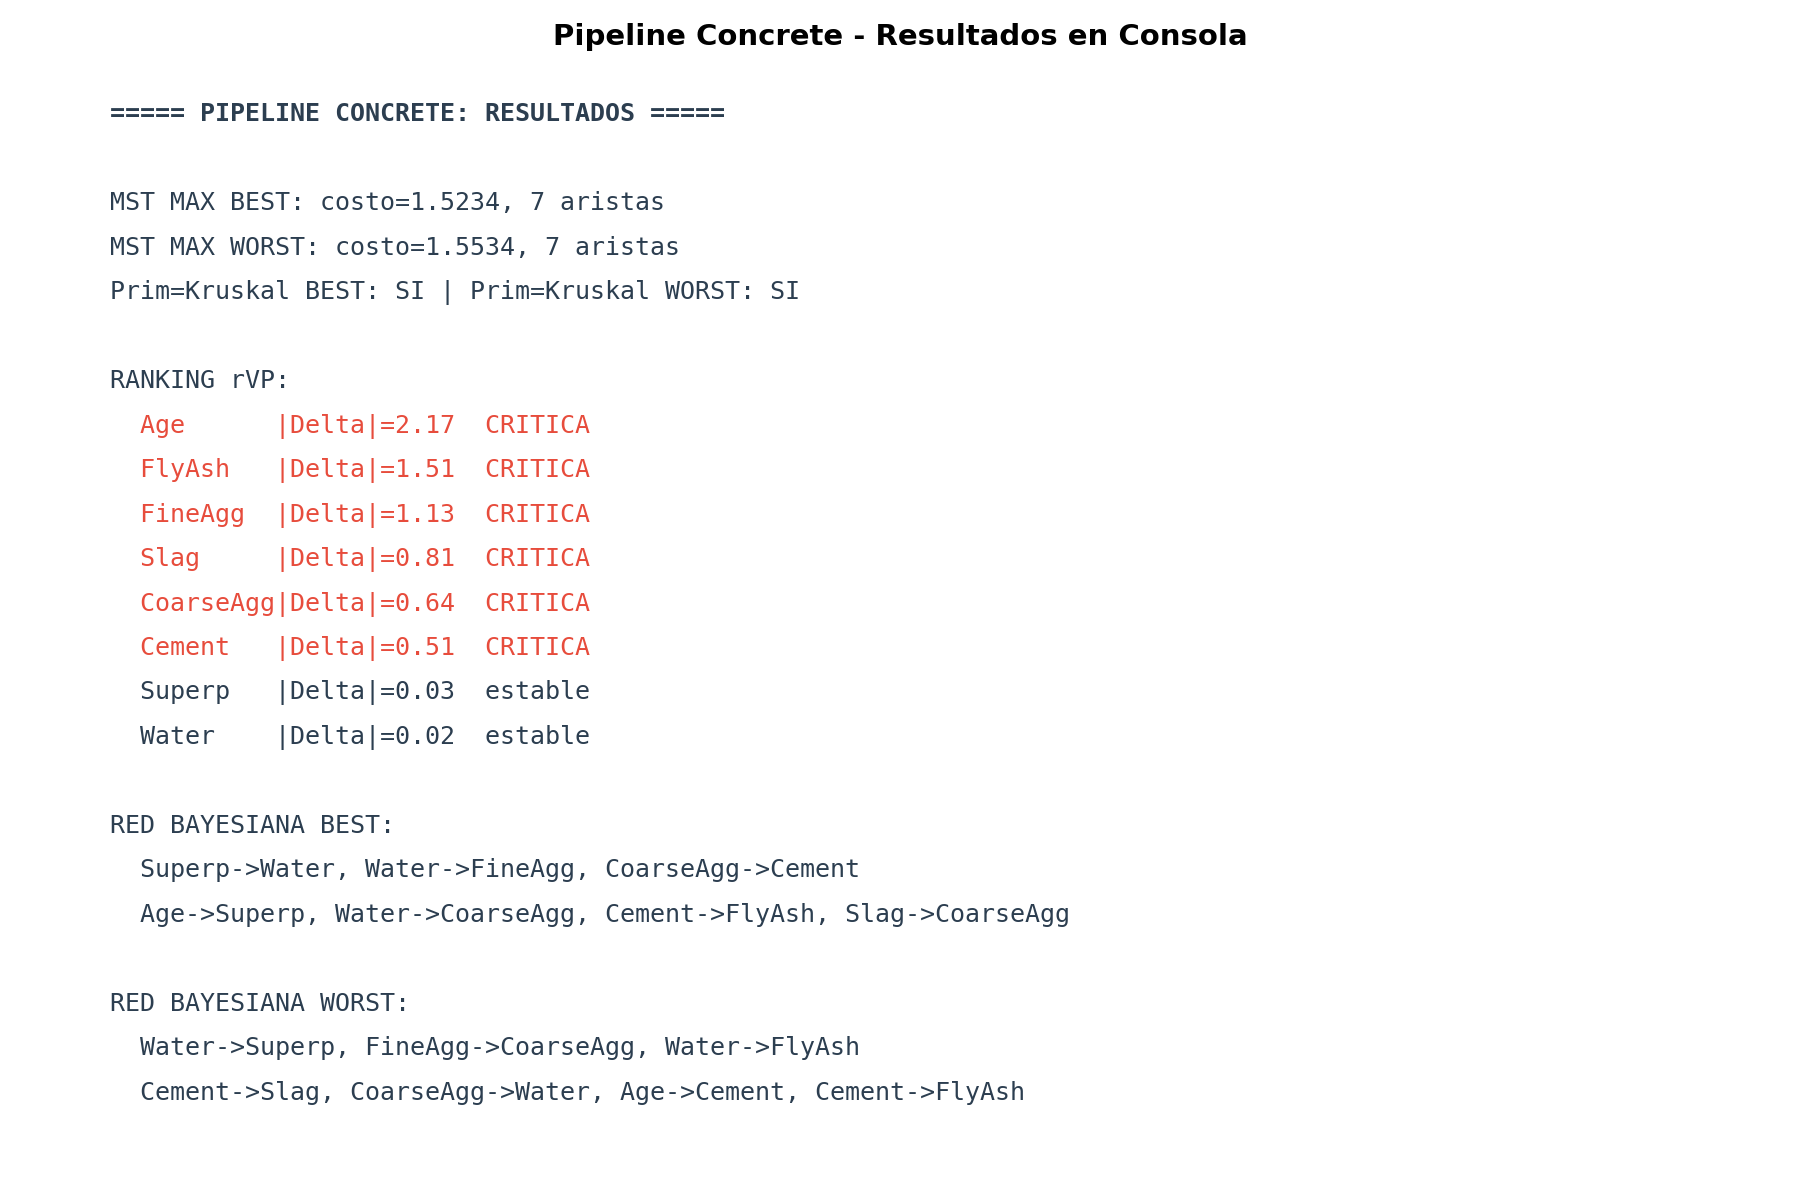
\includegraphics[width=0.75\textwidth]{fig_consola.png}
    \caption{Salida de consola del pipeline completo}
    \label{fig:consola}
\end{figure}

% ==============================================================================
\section*{Referencias}
\addcontentsline{toc}{section}{Referencias}

\begin{thebibliography}{99}

\bibitem{shannon1948}
Shannon, C.~E. (1948).
Una teoria matematica de la comunicacion.
\textit{Bell System Technical Journal}, \textit{27}(3), 379--423.

\bibitem{cover2006}
Cover, T.~M., y Thomas, J.~A. (2006).
\textit{Elementos de teoria de la informacion} (2.\textsuperscript{a} ed.).
Wiley-Interscience.

\bibitem{prim1957}
Prim, R.~C. (1957).
Redes de conexion mas cortas y algunas generalizaciones.
\textit{Bell System Technical Journal}, \textit{36}(6), 1389--1401.

\bibitem{kruskal1956}
Kruskal, J.~B. (1956).
Sobre el subarbol de expansion mas corto de un grafo.
\textit{Proceedings of the AMS}, \textit{7}(1), 48--50.

\bibitem{pearl1988}
Pearl, J. (1988).
\textit{Probabilistic Reasoning in Intelligent Systems}.
Morgan Kaufmann.

\end{thebibliography}

% ==============================================================================
\end{document}
